\documentclass{article}
\usepackage[margin=1in]{geometry}
\usepackage{amsmath}
\usepackage{amssymb}
\usepackage{booktabs}
\usepackage{float}
\usepackage{graphicx}
\usepackage{hyperref}
\usepackage{pdfpages}
\usepackage{siunitx}
\usepackage{adjustbox}
\usepackage{cancel}
\usepackage{paracol}

\usepackage{parskip}

\globalcounter{figure}
\counterwithin{equation}{section}

\title{Report}
\date{23 March 2026}
\author{Connor Emmons}

\begin{document}
\pagenumbering{gobble}
\maketitle
\vfill
\paragraph*{Notes}

\newpage
\pagenumbering{arabic}

\tableofcontents

\newpage

\section{Back to the Drawing Board - Removing Thrust as a Control}

\subsection{Put Cross Product Evaluation as Discrete Constraint}

\subsubsection{Setup}

\begin{itemize}
    \item Objective: $W_{cf} = W_c = 1$
    \begin{itemize}
        \item $J = W_{cf}\left(C_f - C^*\right)^2 + \int_{0}^{t_f}{W_c\left(C - C^*\right)^2dt}$
    \end{itemize}
    \item Constraints: Let $\left[\begin{matrix}c_1&c_2&c_3\\\end{matrix}\right] = \vec{v}_i\times\vec{v}_f;\ \epsilon = \num{1e-3}$
    \begin{itemize}
        \item $x_f - x_i = 0$
        \item $y_f - y_i = 0$
        \item $z_f - z_i = 0$
        \item $\left|c_1\right| \leq \epsilon$
        \item $\left|c_2\right| \leq \epsilon$
        \item $\left|c_3\right| \leq \epsilon$
    \end{itemize}
    \item Bounds:
    \begin{itemize}
        \item $t_0 = 0$
    \end{itemize}
    \item Mesh:
    \begin{itemize}
        \item Segments: 100
        \item Points: 10
    \end{itemize}
    \item Ipopt Options:
    \begin{itemize}
        \item ipopt\_options.tol: \num{1e-8}
    \end{itemize}
\end{itemize}

\subsubsection{Results}

\begin{itemize}
    \item Period Error:
    \begin{itemize}
        \item 158.05 [s]
        \item 0.004087 [\%]
    \end{itemize}
    \item Jacobi Constant/Hamiltonian Deviation:
    \begin{itemize}
        \item Maximum: \num{1.8987e-10}
        \item From $C^*$: \num{1.3831e-8}
    \end{itemize}
    \item Hamiltonian Deviation:
    \begin{itemize}
        \item Maximum: \num{5.8505e-9}
    \end{itemize}
    \item Solution Run Time:
    \begin{itemize}
        \item 28.0 [s]
    \end{itemize}  
\end{itemize}

\newpage

\subsubsection{Plots}

\begin{paracol}{2}

    \begin{figure}[H]
        \centering
        \includegraphics[width=\columnwidth]{no_control_1/orbit.png}
        \caption{2D Representation of Orbit (xy-plane)}
    \end{figure}

    \switchcolumn

    \begin{figure}[H]
        \centering
        \includegraphics[width=\columnwidth]{no_control_1/orbit_ticks.png}
        \caption{2D Representation of Orbit with Day Ticks(xy-plane)}
    \end{figure}

    \switchcolumn

    \begin{figure}[H]
        \centering
        
\includegraphics[width=\columnwidth]{no_control_1/jacobi.png}
        \caption{Jacobi Constant over Orbit}
    \end{figure}

    \switchcolumn

    \begin{figure}[H]
        \centering
        
\includegraphics[width=\columnwidth]{no_control_1/hamiltonian.png}
        \caption{Hamiltonian over Orbit}
    \end{figure}
    
\end{paracol}

\newpage

\begin{figure}[H]
    \centering
    
\includegraphics[width=\columnwidth]{no_control_1/orbit_3D.png}
    \caption{3D Representation of Orbit}
\end{figure}

\newpage

\subsection{Remove the Integral}

\subsubsection{Setup}

\begin{itemize}
    \item Objective: $W_{cf} = 1$
    \begin{itemize}
        \item $J = W_{cf}\left(C_f - C^*\right)^2$
    \end{itemize}
    \item Constraints: Let $\left[\begin{matrix}c_1&c_2&c_3\\\end{matrix}\right] = \vec{v}_i\times\vec{v}_f;\ \epsilon = \num{1e-3}$
    \begin{itemize}
        \item $x_f - x_i = 0$
        \item $y_f - y_i = 0$
        \item $z_f - z_i = 0$
        \item $\left|c_1\right| \leq \epsilon$
        \item $\left|c_2\right| \leq \epsilon$
        \item $\left|c_3\right| \leq \epsilon$
    \end{itemize}
    \item Bounds:
    \begin{itemize}
        \item $t_0 = 0$
    \end{itemize}
    \item Mesh:
    \begin{itemize}
        \item Segments: 100
        \item Points: 10
    \end{itemize}
    \item Ipopt Options:
    \begin{itemize}
        \item ipopt\_options.tol: \num{1e-8}
    \end{itemize}
\end{itemize}

\subsubsection{Results}

\begin{itemize}
    \item Period Error:
    \begin{itemize}
        \item 158.05 [s]
        \item 0.004087 [\%]
    \end{itemize}
    \item Jacobi Constant/Hamiltonian Deviation:
    \begin{itemize}
        \item Maximum: \num{1.8987e-10}
        \item From $C^*$: \num{1.3855e-8}
    \end{itemize}
    \item Hamiltonian Deviation:
    \begin{itemize}
        \item Maximum: \num{5.3502e-10}
    \end{itemize}
    \item Solution Run Time:
    \begin{itemize}
        \item 14.4 [s]
    \end{itemize}  
\end{itemize}

\newpage

\subsubsection{Plots}

\begin{paracol}{2}

    \begin{figure}[H]
        \centering
        \includegraphics[width=\columnwidth]{no_control_2/orbit.png}
        \caption{2D Representation of Orbit (xy-plane)}
    \end{figure}

    \switchcolumn

    \begin{figure}[H]
        \centering
        \includegraphics[width=\columnwidth]{no_control_2/orbit_ticks.png}
        \caption{2D Representation of Orbit with Day Ticks(xy-plane)}
    \end{figure}

    \switchcolumn

    \begin{figure}[H]
        \centering
        
\includegraphics[width=\columnwidth]{no_control_2/jacobi.png}
        \caption{Jacobi Constant over Orbit}
    \end{figure}

    \switchcolumn

    \begin{figure}[H]
        \centering
        
\includegraphics[width=\columnwidth]{no_control_2/hamiltonian.png}
        \caption{Hamiltonian over Orbit}
    \end{figure}
    
\end{paracol}

\newpage

\begin{figure}[H]
    \centering
    
\includegraphics[width=\columnwidth]{no_control_2/orbit_3D.png}
    \caption{3D Representation of Orbit}
\end{figure}

\newpage

\subsection{No Optimization}

\subsubsection{Setup}

\begin{itemize}
    \item Objective:
    \begin{itemize}
        \item $J = 0$
    \end{itemize}
    \item Constraints: Let $\left[\begin{matrix}c_1&c_2&c_3\\\end{matrix}\right] = \vec{v}_i\times\vec{v}_f;\ \epsilon = \num{1e-3}$
    \begin{itemize}
        \item $x_f - x_i = 0$
        \item $y_f - y_i = 0$
        \item $z_f - z_i = 0$
        \item $\left|c_1\right| \leq \epsilon$
        \item $\left|c_2\right| \leq \epsilon$
        \item $\left|c_3\right| \leq \epsilon$
    \end{itemize}
    \item Bounds:
    \begin{itemize}
        \item $t_0 = 0$
    \end{itemize}
    \item Mesh:
    \begin{itemize}
        \item Segments: 100
        \item Points: 10
    \end{itemize}
    \item Ipopt Options:
    \begin{itemize}
        \item ipopt\_options.tol: \num{1e-8}
    \end{itemize}
\end{itemize}

\subsubsection{Results}

\begin{itemize}
    \item Period Error:
    \begin{itemize}
        \item 158.04 [s]
        \item 0.004087 [\%]
    \end{itemize}
    \item Jacobi Constant/Hamiltonian Deviation:
    \begin{itemize}
        \item Maximum: \num{1.8987e-10}
        \item From $C^*$: \num{1.3865e-8}
    \end{itemize}
    \item Hamiltonian Deviation:
    \begin{itemize}
        \item Maximum: \num{1.1635e-12}
    \end{itemize}
    \item Solution Run Time:
    \begin{itemize}
        \item 19.0 [s]
    \end{itemize}  
\end{itemize}

\newpage

\subsubsection{Plots}

\begin{paracol}{2}

    \begin{figure}[H]
        \centering
        \includegraphics[width=\columnwidth]{no_control_3/orbit.png}
        \caption{2D Representation of Orbit (xy-plane)}
    \end{figure}

    \switchcolumn

    \begin{figure}[H]
        \centering
        \includegraphics[width=\columnwidth]{no_control_3/orbit_ticks.png}
        \caption{2D Representation of Orbit with Day Ticks(xy-plane)}
    \end{figure}

    \switchcolumn

    \begin{figure}[H]
        \centering
        
\includegraphics[width=\columnwidth]{no_control_3/jacobi.png}
        \caption{Jacobi Constant over Orbit}
    \end{figure}

    \switchcolumn

    \begin{figure}[H]
        \centering
        
\includegraphics[width=\columnwidth]{no_control_3/hamiltonian.png}
        \caption{Hamiltonian over Orbit}
    \end{figure}
    
\end{paracol}

\newpage

\begin{figure}[H]
    \centering
    
\includegraphics[width=\columnwidth]{no_control_3/orbit_3D.png}
    \caption{3D Representation of Orbit}
\end{figure}

\newpage

\subsection{Minimize Final Time}

\subsubsection{Setup}

\begin{itemize}
    \item Objective:
    \begin{itemize}
        \item $J = t_f$
    \end{itemize}
    \item Constraints: Let $\left[\begin{matrix}c_1&c_2&c_3\\\end{matrix}\right] = \vec{v}_i\times\vec{v}_f;\ \epsilon = \num{1e-3}$
    \begin{itemize}
        \item $x_f - x_i = 0$
        \item $y_f - y_i = 0$
        \item $z_f - z_i = 0$
        \item $\left|c_1\right| \leq \epsilon$
        \item $\left|c_2\right| \leq \epsilon$
        \item $\left|c_3\right| \leq \epsilon$
    \end{itemize}
    \item Bounds:
    \begin{itemize}
        \item $t_0 = 0$
    \end{itemize}
    \item Mesh:
    \begin{itemize}
        \item Segments: 100
        \item Points: 10
    \end{itemize}
    \item Ipopt Options:
    \begin{itemize}
        \item ipopt\_options.tol: \num{1e-8}
    \end{itemize}
\end{itemize}

\subsubsection{Results}

\begin{itemize}
    \item Period Error:
    \begin{itemize}
        \item 2922571.01 [s]
        \item 75.5825 [\%]
    \end{itemize}
    \item Jacobi Constant/Hamiltonian Deviation:
    \begin{itemize}
        \item Maximum: \num{80.0983}
        \item From $C^*$: \num{0.5044}
    \end{itemize}
    \item Hamiltonian Deviation:
    \begin{itemize}
        \item Maximum: \num{622.3424}
    \end{itemize}
    \item Solution Run Time:
    \begin{itemize}
        \item 4 [min] 12.5 [s]
    \end{itemize}  
\end{itemize}

\newpage

\subsubsection{Plots}

\begin{paracol}{2}

    \begin{figure}[H]
        \centering
        
\includegraphics[width=\columnwidth]{no_control_4/orbit.png}
        \caption{2D Representation of Orbit (xy-plane)}
    \end{figure}

    \switchcolumn

    \begin{figure}[H]
        \centering
        
\includegraphics[width=\columnwidth]{no_control_4/orbit_ticks.png}
        \caption{2D Representation of Orbit with Day Ticks(xy-plane)}
    \end{figure}

    \switchcolumn

    \begin{figure}[H]
        \centering
        
\includegraphics[width=\columnwidth]{no_control_4/jacobi.png}
        \caption{Jacobi Constant over Orbit}
    \end{figure}

    \switchcolumn

    \begin{figure}[H]
        \centering
        
\includegraphics[width=\columnwidth]{no_control_4/hamiltonian.png}
        \caption{Hamiltonian over Orbit}
    \end{figure}
    
\end{paracol}

\newpage

\begin{figure}[H]
    \centering
    
\includegraphics[width=\columnwidth]{no_control_4/orbit_3D.png}
    \caption{3D Representation of Orbit}
\end{figure}

\newpage

\subsection{Cross Product as Objective}

\subsubsection{Setup}

\begin{itemize}
    \item Objective: Let $\left[\begin{matrix}c_1&c_2&c_3\\\end{matrix}\right] = \vec{v}_i\times\vec{v}_f$
    \begin{itemize}
        \item $J = W_{cf}\left(C_f - C^*\right)^2 + W_v\left(c_1^2 + c_2^2 + c_3^2\right)$
    \end{itemize}
    \item Constraints: 
    \begin{itemize}
        \item $x_f - x_i = 0$
        \item $y_f - y_i = 0$
        \item $z_f - z_i = 0$
    \end{itemize}
    \item Bounds:
    \begin{itemize}
        \item $t_0 = 0$
    \end{itemize}
    \item Mesh:
    \begin{itemize}
        \item Segments: 100
        \item Points: 10
    \end{itemize}
    \item Ipopt Options:
    \begin{itemize}
        \item ipopt\_options.tol: \num{1e-8}
    \end{itemize}
\end{itemize}

\subsubsection{Results}

\begin{itemize}
    \item Period Error:
    \begin{itemize}
        \item 142.60 [s]
        \item 0.003688 [\%]
    \end{itemize}
    \item Jacobi Constant/Hamiltonian Deviation:
    \begin{itemize}
        \item Maximum: \num{1.8987e-10}
        \item From $C^*$: \num{9.9576e-8}
    \end{itemize}
    \item Hamiltonian Deviation:
    \begin{itemize}
        \item Maximum: \num{1.8659e-7}
    \end{itemize}
    \item Solution Run Time:
    \begin{itemize}
        \item 8.9 [s]
    \end{itemize}  
\end{itemize}

\newpage

\subsubsection{Plots}

\begin{paracol}{2}

    \begin{figure}[H]
        \centering
        
\includegraphics[width=\columnwidth]{no_control_5/orbit.png}
        \caption{2D Representation of Orbit (xy-plane)}
    \end{figure}

    \switchcolumn

    \begin{figure}[H]
        \centering
        
\includegraphics[width=\columnwidth]{no_control_5/orbit_ticks.png}
        \caption{2D Representation of Orbit with Day Ticks(xy-plane)}
    \end{figure}

    \switchcolumn

    \begin{figure}[H]
        \centering
        
\includegraphics[width=\columnwidth]{no_control_5/jacobi.png}
        \caption{Jacobi Constant over Orbit}
    \end{figure}

    \switchcolumn

    \begin{figure}[H]
        \centering
        
\includegraphics[width=\columnwidth]{no_control_5/hamiltonian.png}
        \caption{Hamiltonian over Orbit}
    \end{figure}
    
\end{paracol}

\newpage

\begin{figure}[H]
    \centering
    
\includegraphics[width=\columnwidth]{no_control_5/orbit_3D.png}
    \caption{3D Representation of Orbit}
\end{figure}

\newpage

\subsection{Cross Product Only}

\subsubsection{Setup}

\begin{itemize}
    \item Objective: Let $\left[\begin{matrix}c_1&c_2&c_3\\\end{matrix}\right] = \vec{v}_i\times\vec{v}_f$
    \begin{itemize}
        \item $J = W_v\left(c_1^2 + c_2^2 + c_3^2\right)$
    \end{itemize}
    \item Constraints: 
    \begin{itemize}
        \item $x_f - x_i = 0$
        \item $y_f - y_i = 0$
        \item $z_f - z_i = 0$
    \end{itemize}
    \item Bounds:
    \begin{itemize}
        \item $t_0 = 0$
    \end{itemize}
    \item Mesh:
    \begin{itemize}
        \item Segments: 100
        \item Points: 10
    \end{itemize}
    \item Ipopt Options:
    \begin{itemize}
        \item ipopt\_options.tol: \num{1e-8}
    \end{itemize}
\end{itemize}

\subsubsection{Results}

\begin{itemize}
    \item Period Error:
    \begin{itemize}
        \item 142.60 [s]
        \item 0.003688 [\%]
    \end{itemize}
    \item Jacobi Constant/Hamiltonian Deviation:
    \begin{itemize}
        \item Maximum: \num{1.8988e-10}
        \item From $C^*$: \num{9.9635e-8}
    \end{itemize}
    \item Hamiltonian Deviation:
    \begin{itemize}
        \item Maximum: \num{1.8296e-7}
    \end{itemize}
    \item Solution Run Time:
    \begin{itemize}
        \item 10.9 [s]
    \end{itemize}  
\end{itemize}

\newpage

\subsubsection{Plots}

\begin{paracol}{2}

    \begin{figure}[H]
        \centering
        
\includegraphics[width=\columnwidth]{no_control_6/orbit.png}
        \caption{2D Representation of Orbit (xy-plane)}
    \end{figure}

    \switchcolumn

    \begin{figure}[H]
        \centering
        
\includegraphics[width=\columnwidth]{no_control_6/orbit_ticks.png}
        \caption{2D Representation of Orbit with Day Ticks(xy-plane)}
    \end{figure}

    \switchcolumn

    \begin{figure}[H]
        \centering
        
\includegraphics[width=\columnwidth]{no_control_6/jacobi.png}
        \caption{Jacobi Constant over Orbit}
    \end{figure}

    \switchcolumn

    \begin{figure}[H]
        \centering
        
\includegraphics[width=\columnwidth]{no_control_6/hamiltonian.png}
        \caption{Hamiltonian over Orbit}
    \end{figure}
    
\end{paracol}

\newpage

\begin{figure}[H]
    \centering
    
\includegraphics[width=\columnwidth]{no_control_6/orbit_3D.png}
    \caption{3D Representation of Orbit}
\end{figure}

\newpage

\subsection{Notes}

\begin{itemize}
    \item The integral of the difference in Jacobi constant only hurts performance - good idea, but not necessary with cross product constraint
    \item Objective as just final Jacobi constant or nothing at all both work, keeping the final Jacobi just to have something to minimize seems better
    \item Minimum time is a trap
    \item Putting the cross product in the objective instead of in the constraints seems to work well
    \item Best option for exploring 3D orbits is probably having only the cross product in the objective and not the final Jacobi constant
\end{itemize}

\section{Generating Tilted Orbits for (1,1) Cyclers}

\subsection{45 Degree Guess}

\subsubsection{Setup}

\begin{itemize}
    \item Objective: Let $\left[\begin{matrix}c_1&c_2&c_3\\\end{matrix}\right] = \vec{v}_i\times\vec{v}_f$
    \begin{itemize}
        \item $J = W_v\left(c_1^2 + c_2^2 + c_3^2\right)$
    \end{itemize}
    \item Constraints: 
    \begin{itemize}
        \item $x_f - x_i = 0$
        \item $y_f - y_i = 0$
        \item $z_f - z_i = 0$
    \end{itemize}
    \item Bounds:
    \begin{itemize}
        \item $t_0 = 0$
    \end{itemize}
    \item Mesh:
    \begin{itemize}
        \item Segments: 100
        \item Points: 10
    \end{itemize}
    \item Ipopt Options:
    \begin{itemize}
        \item ipopt\_options.tol: \num{1e-8}
    \end{itemize}
    \item Initial Guess: Take the planar cycler generated from the approach using the cross product as the objective and nothing else and rotate the entire orbit about the x-axis by exactly 45 degrees.
\end{itemize}

\subsubsection{Results}

\begin{itemize}
    \item Jacobi Constant/Hamiltonian Deviation:
    \begin{itemize}
        \item Maximum: \num{1.5788e-10}
    \end{itemize}
    \item Hamiltonian Deviation:
    \begin{itemize}
        \item Maximum: \num{9.6679e-9}
    \end{itemize}
    \item Solution Run Time:
    \begin{itemize}
        \item 6.8 [s]
    \end{itemize}  
\end{itemize}

\newpage

\subsubsection{Plots}

\begin{paracol}{2}

    \begin{figure}[H]
        \centering
        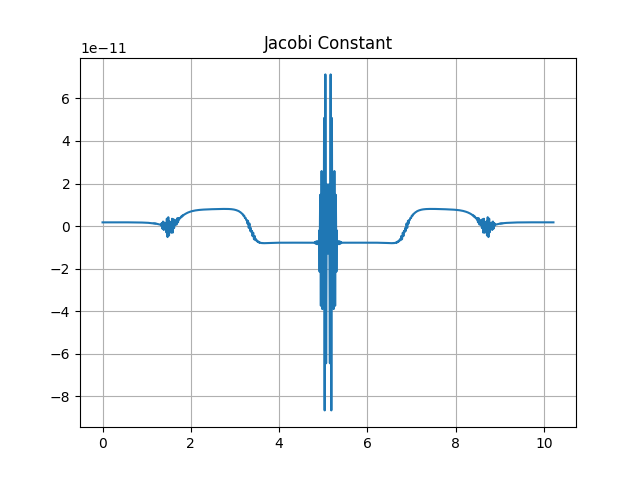
\includegraphics[width=\columnwidth]{3D_1/jacobi.png}
        \caption{Jacobi Constant over Orbit}
    \end{figure}

    \switchcolumn

    \begin{figure}[H]
        \centering
        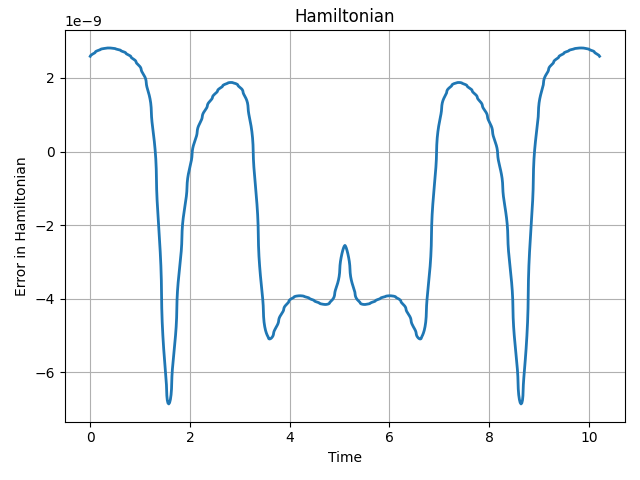
\includegraphics[width=\columnwidth]{3D_1/hamiltonian.png}
        \caption{Hamiltonian over Orbit}
    \end{figure}
    
\end{paracol}

\begin{figure}[H]
    \centering
    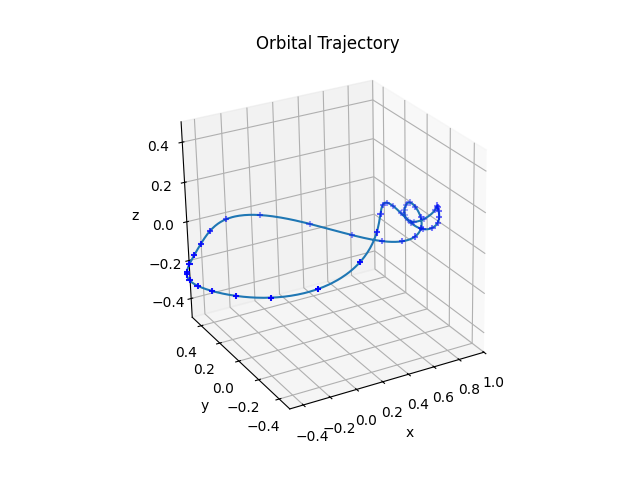
\includegraphics[width=\columnwidth]{3D_1/orbit_3D.png}
    \caption{3D Representation of Orbit}
\end{figure}

\newpage

\subsection{60 degree Guess}

\subsubsection{Setup}

\begin{itemize}
    \item Objective: Let $\left[\begin{matrix}c_1&c_2&c_3\\\end{matrix}\right] = \vec{v}_i\times\vec{v}_f$
    \begin{itemize}
        \item $J = W_v\left(c_1^2 + c_2^2 + c_3^2\right)$
    \end{itemize}
    \item Constraints: 
    \begin{itemize}
        \item $x_f - x_i = 0$
        \item $y_f - y_i = 0$
        \item $z_f - z_i = 0$
    \end{itemize}
    \item Bounds:
    \begin{itemize}
        \item $t_0 = 0$
    \end{itemize}
    \item Mesh:
    \begin{itemize}
        \item Segments: 100
        \item Points: 10
    \end{itemize}
    \item Ipopt Options:
    \begin{itemize}
        \item ipopt\_options.tol: \num{1e-8}
    \end{itemize}
    \item Initial Guess: Take the planar cycler generated from the approach using the cross product as the objective and nothing else and rotate the entire orbit about the x-axis by exactly 45 degrees.
\end{itemize}

\subsubsection{Results}

\begin{itemize}
    \item Jacobi Constant/Hamiltonian Deviation:
    \begin{itemize}
        \item Maximum: \num{8.6509e-13}
    \end{itemize}
    \item Hamiltonian Deviation:
    \begin{itemize}
        \item Maximum: \num{2.3155e-10}
    \end{itemize}
    \item Solution Run Time:
    \begin{itemize}
        \item 10.5 [s]
    \end{itemize}  
\end{itemize}

\newpage

\subsubsection{Plots}

\begin{paracol}{2}

    \begin{figure}[H]
        \centering
        
\includegraphics[width=\columnwidth]{3D_2/jacobi.png}
        \caption{Jacobi Constant over Orbit}
    \end{figure}

    \switchcolumn

    \begin{figure}[H]
        \centering
        
\includegraphics[width=\columnwidth]{3D_2/hamiltonian.png}
        \caption{Hamiltonian over Orbit}
    \end{figure}
    
\end{paracol}

\begin{figure}[H]
    \centering
    
\includegraphics[width=\columnwidth]{3D_2/orbit_3D.png}
    \caption{3D Representation of Orbit}
\end{figure}

\newpage

\subsection{30 Degree Guess}

\subsubsection{Setup}

\begin{itemize}
    \item Objective: Let $\left[\begin{matrix}c_1&c_2&c_3\\\end{matrix}\right] = \vec{v}_i\times\vec{v}_f$
    \begin{itemize}
        \item $J = W_v\left(c_1^2 + c_2^2 + c_3^2\right)$
    \end{itemize}
    \item Constraints: 
    \begin{itemize}
        \item $x_f - x_i = 0$
        \item $y_f - y_i = 0$
        \item $z_f - z_i = 0$
    \end{itemize}
    \item Bounds:
    \begin{itemize}
        \item $t_0 = 0$
    \end{itemize}
    \item Mesh:
    \begin{itemize}
        \item Segments: 100
        \item Points: 10
    \end{itemize}
    \item Ipopt Options:
    \begin{itemize}
        \item ipopt\_options.tol: \num{1e-8}
    \end{itemize}
    \item Initial Guess: Take the planar cycler generated from the approach using the cross product as the objective and nothing else and rotate the entire orbit about the x-axis by exactly 45 degrees.
\end{itemize}

\subsubsection{Results}

\begin{itemize}
    \item Jacobi Constant/Hamiltonian Deviation:
    \begin{itemize}
        \item Maximum: \num{1.5788e-10}
    \end{itemize}
    \item Hamiltonian Deviation:
    \begin{itemize}
        \item Maximum: \num{9.6679e-9}
    \end{itemize}
    \item Solution Run Time:
    \begin{itemize}
        \item 6.8 [s]
    \end{itemize}  
\end{itemize}

\newpage

\subsubsection{Plots}

\begin{paracol}{2}

    \begin{figure}[H]
        \centering
        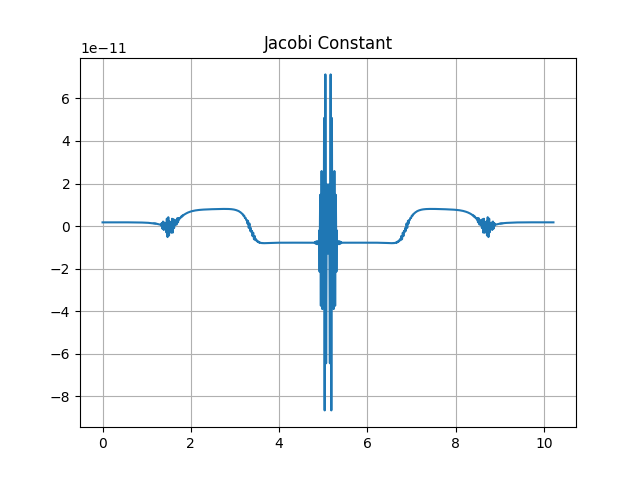
\includegraphics[width=\columnwidth]{3D_1/jacobi.png}
        \caption{Jacobi Constant over Orbit}
    \end{figure}

    \switchcolumn

    \begin{figure}[H]
        \centering
        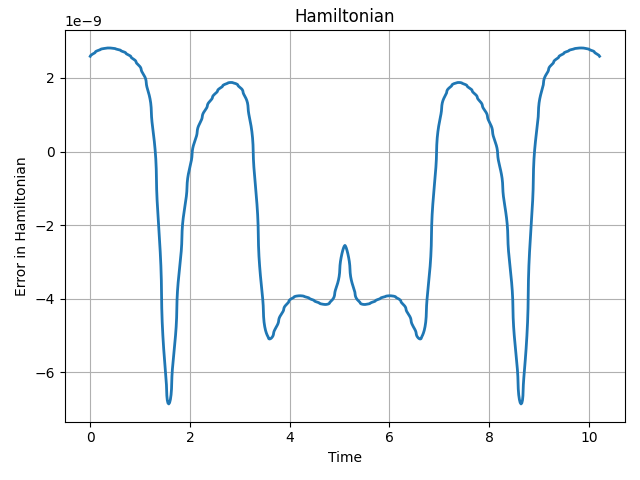
\includegraphics[width=\columnwidth]{3D_1/hamiltonian.png}
        \caption{Hamiltonian over Orbit}
    \end{figure}
    
\end{paracol}

\begin{figure}[H]
    \centering
    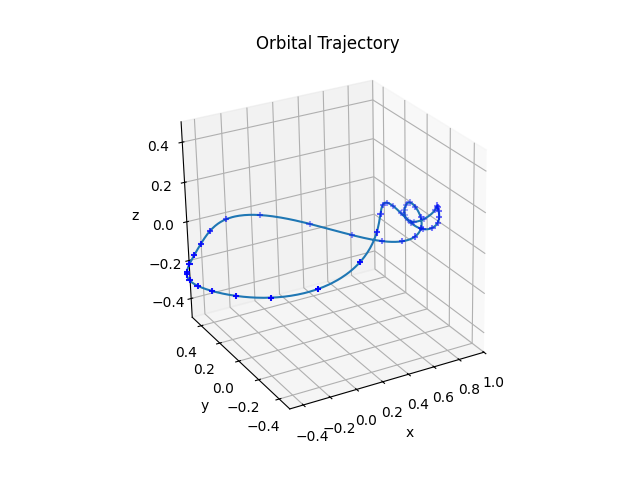
\includegraphics[width=\columnwidth]{3D_1/orbit_3D.png}
    \caption{3D Representation of Orbit}
\end{figure}

\newpage

\subsection{Notes}

The 45 degree guess produced a feasible inclined orbit, and the 60 degree guess produced an orbit which is not inclined, but is also feasible and potentially indicates a family of pseudocyclers. Next steps are to perform an angle sweep to find out which angles give good orbits, recycling the solutions as guesses up to 90 degrees of inclination. The problem setup is much better, yielding better results with significantly decreased run times. After the angle sweep, plan is to look into other cycler families and solar perturbations.

\end{document}